\section{Prerequisites of Thermodynamics}
\notedate{(I) THU 29/09/2022}
In thermodynamics there are \textbf{extensive} quantities, that grows with the system size, and \textbf{intensive} quantities, which does not. \textbf{Conjugation} between them, means \textit{tuning} intensive variables to make extensive one change.

\gray{Note that we always refer to quasi-static transformations}

\subsection{The laws of thermodynamics}
\textbf{0th Law} Equilibrium (empirical) temperature.\\

We call: \qquad $\mathcal{M}_A$ : space of state of $A$\qquad
$\mathcal{M}_B$ : space of state of $B$.\\
The total phase space is $\mathcal{M}_A \times \mathcal{M}_B = \{(a,b)\}$,   where $(a,b)$ denotes all possible couples.\\

At equilibrium, not all couples are possible. At equilibrium:
$$
    F_{AB}(a,b) = 0 \iff (a,b)
$$
so there is a constraint. This is an equivalence relation:
$$
    A\sim A \qquad A \sim B \iff B \sim A \qquad A \sim B \ \& \  B\sim C \implies A\sim C
$$  
$$
    F_{AB}(a,b) = f_A(a) - f_B(b) = 0
$$
This condition define the \textit{empirical temperature} $t_A = t_B$ at equilibrium.

\gray{The transitive property allow us to choose anything as a measure (e.g. thermometer).}\\

\textbf{1st Law} Internal energy $E$\\

There is an internal energy, which can change in different ways, but it always conserved (\textit{conservation of energy}).
$$ dE = \delta Q - \delta  \mathcal{L} + \mu dN $$

where $\delta Q$ is heat, $\delta \work$ is work, $N$ is number of particles and $\mu$ is the chemical potential: the energy needed to add/remove a particle.\\

\gray{$d$ means that $\oint dE = 0$ on any cycle, so the integral does not depend on the path.\qquad  $\delta$ no, so $\delta Q, \delta \work$ is not necessary 0.}\\

E.g. Classical fluids:\\
$\delta\work = pdV$ : the work derive from the compression/expansion. So the variation of the energy: $dE = \delta Q - pdV + \mu dN$.

\textbf{2nd Law} Entropy $S$\\

In a reversible process: 
$$ \oint \frac{\delta Q}T = 0 \qquad \text{in general:} \quad \frac{delta Q}T = dS$$

Putting the two laws together,
$$ \oint \frac{\delta Q}T \le 0 \implies dS \ge \frac{\delta Q}T \quad (= 0 \text{ for reversible)}$$ 

So, \textbf{a system evolves towards the maximum of entropy}\\

\textbf{3rd Law} For any isothermal process, $\Delta S \xrightarrow[T\to 0]{}0$

\subsection{Thermodynamic potentials (for reversible processes)}
Let's see the relation between these quantities:

\textbf{Internal energy} $dE = TdS - pdV + \mu dN$\\
The internal energy can be changed by changing $S, V, N$ so $E = E(S,V,N)$ and:
$$ T = \left.\frac{\partial E}{\partial S}\right|_{V,N} \qquad
   p = -\left.\frac{\partial E}{\partial V}\right|_{S,N} \qquad
   \mu = \left.\frac{\partial E}{\partial N}\right|_{S,V} \qquad
$$

\gray{All terms in couple are conjugate variables: $T \lrarr S, p\lrarr V, \mu \lrarr N$}

$E, S, V, N$ are extensive variables, so if 
$$ \begin{cases}N \rightarrow \lambda N\\V \rightarrow \lambda V\\S \rightarrow \lambda S\end{cases} \implies E = \lambda E
$$
where $\lambda$ is a scaling factor.

So:
$$ \boxed{E(\lambda S, \lambda V, \lambda N) = \lambda E(S,V,N) }$$
Homogeneous function of degree 1 (linear)

That requires: $E(S,V,N) = TS - pV + \mu N \qquad dE = TdS - pdV + \mu dN$\\

Usually it's easier to work with $T$ then $S$ (there are no experiment where you can tune the entropy $S$), so thermodynamic potentials are introduced. These are other function which are more convenient to work with:

\begin{itemize}
    \item Internal energy:\\
    $E(S,V,N) = TS - pV + \mu N \qquad\qquad dE = TdS - pdV + \mu dN$
    \item Helmotz free energy:\\
    $F(T,V,N) = E - TS = -pV + \mu N \qquad\qquad dF = -SdT - pdV + \mu dN$
    \item Entalpy:\\
    $H(S,p,N) = E+ pV = ST + \mu N \qquad\qquad dH = TdS + Vdp + \mu dN$
    \item Gibbs free energy:\\
    $G(T,p,V) = E- TS + pV = \mu N \qquad\qquad dG = -SdT + Vdp + \mu dN$
    \item Granpotential:\\
    $\Omega(T,V,\mu) = E-TS - \mu N = -pV \qquad\qquad d\Omega = -SdT - pdV - N d\mu$
\end{itemize}

\subsection{Thermodynamic limit}
$N,V \to \infty$ \quad with $n=N/V$ fixed
In this limit, all the thermodynamic potential diverges, so (e.g) $E$ has no meaning. What we can calculate is the ratio with the number of particle (e.g $E/N$ : internal energy for particle). Things do not change because they depend on $N$, except for $\Omega$ which doesn't.
$$ e \equiv \frac EN \qquad s \equiv \frac SN \qquad v \equiv \frac VN \qquad f \equiv \frac FN \qquad g \equiv \frac GN \qquad \omega \equiv \frac \Omega N
$$

\subsection{Equation of state - \texorpdfstring{$\mu$-$n$}{mu-n} relation}
From the granpotential, one can derive $p = -\frac{\partial\Omega}{\partial V}$, which, written for a particular model (e.g. classical gas) gives the \textit{equation of state} of the system/model.

Also, the $\mu$-$n$ relation is very important: $N = -\frac{\partial\Omega}{\partial \mu}$

\subsection{Variational principles}
\notedate{(II) MON 03/10/2022}
Suppose we set up an experiment in which $S,V,N$ are constant. Then $dE = 0$, which implies that the system evolves towards the minimum of energy $E$.\\
The same happen if $T,V,N$ are constant, in which case $dF = 0$, so the system evolves towards the minimum of Helmotz free energy. Etc... .

So the problem becomes a problem of minimization.\\
\gray{We'll see that the minimization of $F$ and $\Omega$ are the most important.}

For reversible processes, $dF = -SdT + pdV + \mu dN$, from which:
$$ S = \left. -\frac{\partial F}{\partial T}\right|_{V,N} \qquad
p = \left. -\frac{\partial F}{\partial V}\right|_{T,N} \qquad
\mu = \left. \frac{\partial F}{\partial T}\right|_{T,V} \qquad
$$

The minimum is found with the hessian matrix:
\begingroup
\renewcommand*{\arraystretch}{2.5}

$$\hess (F) = \begin{pmatrix} 
\dfrac{\partial^2 F}{\partial T ^2} & \dfrac{\partial^2 F}{\partial T \partial V} & \dfrac{\partial^2 F}{\partial T \partial N} \\
\dfrac{\partial^2 F}{\partial V \partial T} & \dfrac{\partial^2 F}{\partial V^2} & \dfrac{\partial^2 F}{\partial V \partial N} \\
\dfrac{\partial^2 F}{\partial N \partial T} & \dfrac{\partial^2 F}{\partial N \partial V} & \dfrac{\partial^2 F}{\partial N^2}
\end{pmatrix}$$
\endgroup
In fact, the condition to have a minimum is that all the 3 eigenvalues of the hessian matrix should be $>0$.

\gray{That is the same as saying that going in every direction the "gradient" increase}

We won't prove this, but because of the way $ F = F(T,V,N)$, it us sufficient that
$$ \frac{\partial ^2 F}{\partial T^2} < 0 \qquad
\frac{\partial ^2 F}{\partial V^2} > 0 \qquad 
\frac{\partial ^2 F}{\partial T\partial N} \le 0 \qquad 
$$

\gray{The same can be done changing the variables and it also works with other different from F (e.g. $E$ etc.)}

\section{Prerequisites of Classical Mechanics}
To represent a classical system we need:\\

\textbf{1) Coordinates:} position $q$, momenta $p$.\\
\gray{For 1 particle. If a particle lives in $\R^d \implies \vec q \in \R^d \quad \vec p \in \R^d$.}\\
So the phase space $\ps_1$ is $\{(q,p)\} \in \R^d \times R^d = 2\R^d$\\

For N particles living in $\R^d$, the phase space is:
$$\ps_N = \{(q_1,p_1, q_2, p_2, \dots, q_n,p_N)\} = \{(q_i,p_i)\quad i = 1,\dots, N\} = \R^{2dN}
$$

\textbf{2) Observable:} An observable is given by a smooth real function from the phase space to a real number.
$$f(q_i,p_i) : \ps_N \to \R$$
\gray{e.g. $\ham$, angular momentum, kinetic energy $T$ are all observables}\\

\textbf{3) Measure:} (ideal, without errors) A measure of an observable on a state $(\bar q_i \bar p_i)$ is given by the value of the function at that particular point: $f(\bar q_1, \bar p_1)$\\

\textbf{4) Evolution:} The evolution of a system is fixed by a special observable, called Hamiltonian $\ham$, through Hamilton's \textit{equation of motion}:
\begin{equation} \label{eq:ham}
\dot q_i = \der{\ham}{p_i} \qquad \dot p_i = -\der{\ham}{q_i} \qquad \text{(they give Newton's law)}
\end{equation}

In general, $\ham = \ham(q_i, p_i, t)$, but we only study the case where the hamiltonian is time-independent.\\

The equation \ref{eq:ham} are equation of the first order in $t$ ($q_i(t) p_i(t)$), so the solution is uniquely fixed by the initial conditions $(\bar q_i, \bar p_i)$. Because of that we have two theorems:

\textbf{Conservation of volumes} (even id the shape is changed).
Since each point of the phase space is a state, the volume counts the number of states. In other words, giving a volume is the same as giving a subset.

\textbf{Conservation of energy}. If $\ham$ does not depend explicitly on time, the hamiltonian is constant for each curve of motion:
$$ E= \ham (q_i(t), p_i(t)) = \ham(\bar q_i, \bar p_i) = \ham (q_i(t=0), p_i(t=0))$$ 

\subsection{On the notion of "state"}
We will call one of these states $(q_i(t), p_i(t))$ a \textbf{microstate} at time $t$. Fixing an initial microstate, completely determine the trajectory in phase space, backward and forward in time. 

\gray{If the initial conditions are changed a little, allowing the system to "choose" them between a given set, we enter the field of \textit{complex systems}}

In general, there is a (huge) number of possible microstates corresponding to the same macroscopic set of thermodynamic variables (the \textbf{macrostate}).

In order to study this, we can think of having an \textbf{ensemble}: a large number of copies of the system, all with the same Macroscopic State but with different microscopic realizations.

\subsection{Probability distribution}
Given an ensemble, in the limit in which the number of copies becomes very large, we can construct the probability with which, at a fixed time, a given microstate $\{q_i(t), p_i(t)\}$ appears, thus recovering a \textbf{probability density distribution} on $\ps_N$:
$$\rho(q_i(t), p_i(t)) \qquad \ps_N \to \R^+ (0,1)$$
Which is:
\begin{itemize}
    \item Positive: $\qquad \rho (p_i(t), p_i(t)) \ge 0 $
    \item Normalized: $$ \int_{\ps_N}\rho(q_i,p_i) \left(\prod_{I=1}^N dq_i dp_i\right) = 1$$
    (implicit vector used: $dq_i, dp_i$ should be $d^3\vec q_i, d^3 \vec p_i$)
    \item For a subset $U \subset \ps_N$, the probability to find the system in the subset $U$ is: $\int_U \rho(q_i,p_i) d\Gamma$
\end{itemize}

\hspace{0pt}

To have an a-dimensional quantity, we replace: 
$$ d\Gamma \equiv \prod_i dq_i dp_i \qquad \text{with}\quad  d\Omega \equiv \frac{\prod_i dq_i dp_i}h $$
where $h$ is a constant with the dimension of an action \gray{(here we don't say anything about it, it's just the dimension of a little state of sides $dq_i, dp_i$ but in quantum mechanics, it will be Plank's constant)}.

\subsection{Liouville's theorem}
The conservation of volumes is the Liouville's theorem.\\Given a region $\Omega_0$ in which there is some density probability $\rho(q_i,p_i) \in \Omega_0$, there is a density current $\vec J$ of particles moving out of $\Omega_0$:
$$ \vec J = \rho \vec v \qquad \text{where } \vec v = (\dot q_i, \dot p_i) \text{ is a velocity in phase space}$$

If there is a conservation of the total probability density: $\der\rho t + \vec\nabla(\vec J) = 0$
That means 
$$ \Der \rho t = \der tho t + \vec \nabla(\rho \vec v) = 0$$
which is the Liouville's theorem

We can also use the Poisson's bracket's to write $\vec\nabla(\rho \vec v) = \{\rho, \ham\}$,\\ 
\gray{reminding that $\{f,g\} = \sum_i \left(\der f{q_i}\der g{p_i} - \der g{q_i} \der f{p_i}\right)$}\\

\Def A system is called \textbf{stationary} iff $\der \rho t = 0$. Stationarity is a necessary condition for \textbf{equilibrium}: $\Der \rho t = 0$, which is what we want to study. From the previous condition follows that at equilibrium: $\{\rho,\ham\} = 0$ which can happen if
\begin{enumerate}
    \item $\rho = const$
    \item $\rho = \rho(\ham(q_i,p_i))$
\end{enumerate}
giving, respectively, the cases of the microcanonical and canonical/grancanonical distributions.\\

\Def Given an observable $f$, we can define its: 
\begin{align*}  
\text{\textbf{average}} \qquad& \langle f\rangle_\rho = \int_{\ps_N} f(q_i, p_i) \rho (q_i,p_i) \left(\prod_{i=1}^N \frac {dq_idp_i}h\right) \\
\text{\textbf{standard deviation}} \qquad & (\Delta t)^2 = \langle f^2 \rangle_\rho - (\langle f\rangle_\rho)^2
\end{align*}
\gray{The subscript $_\rho$, indicates that we need to have defined a probability density distribution, to evaluate these two.}

\subsection{Time-Independent Hamiltonians}
\begin{wrapfigure}{r}{0.3\textwidth}
    \centering
    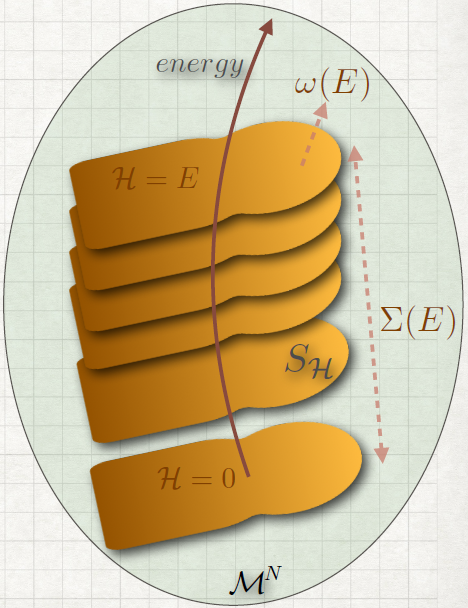
\includegraphics[width=0.29\textwidth]{foliated space.png}
\end{wrapfigure}
For time-independent hamiltonians, the energy is conserved. That means that all the trajectories will be on a $(2M-1)$hypersurface in the phase space (where $M$ is the total number of degree of freedom). The whole space can thus be foliated into different sheets according to different energies like in the figure.

So we can compute every integrals integrating firstly over an hypersurface of constant energy and then over all the possible energies:
$$ \int (\dots) \prod dq_i dp_i = \int_0^\infty d\ham \int_\ham ds_\ham (\dots)$$


\Def Volume ($\sim$ number of state) in phase space with energy lower than a certain value ($0\le\ham(q_i,p_i)\le E$):
$$ \Sigma (E) \equiv \int_{0\le \ham \le E} \prod _i dq_i dp_i = \int_0^E d\ham \int_{S_\ham}dS_\ham = \int_0^E d\ham \omega(\ham)$$

\Def The density of state is the "area" of the hypersurface $S_\ham$
$$ \omega(E) \equiv \int_{S_\ham} dS_\ham= \der\Sigma E$$

\gray{$\Sigma,\omega$ aren't property of the space, but they depends on $\ham$ because the surfaces depend on $\ham$.}\\

In the case of time-independent hamiltonians:
\begin{align*}    
&\angles f _E \equiv \frac1{\omega(E)} \int_{S_E} dS_E f\\
\text{time average}\qquad &\angles f_\infty \equiv \lim_{T\to \infty} \frac 1T \int_{t_0}^{t_0+T} dt f(q_i(t), p_i(t))
\end{align*} 
the latter exists for almost all initial conditions and it is independent of $t_0$

\Def A system is said to be \textbf{ergodic} over the surface $S_E$ iff almost all points $(q_i,p_i) \in S_E$ pass through a neighbourhood $U \in S_E$ during the evolution. In other words, starting from any point, if you let the system evolve for a long time, every region will be explored.

\Th A system is ergodic iff, for almost all initial points: $\angles f_\infty = \angles f_E$\\
This tell that the time spent on a region is proportional to the area of that region. 

\gray{In the following we will consider only ergodic systems.}